%Enhancement: Explain properly this algorithm as a KWIK algorithm
Let $G$ be a network graph with source $s$ and sink $t$ where every edge $(i,j)$ has a cost vector $v_{ij}$ associated to it. Let $w$ be a weight vector. The cost for an agent to traverse the edge $(i,j)$ is $cost(i,j)=w \cdot v_{ij}$. \\

The algorithm knows $G, v_{ij}$ for all edges $(i,j)$  and every time it traverses the edge $(i,j)$ it receives $w \cdot v_{ij}$. However, it doesn't know $w$.  \\

The goal of the algorithm is to find a path from source $s$ to sink $t$ with the lowest for the agent in the fewest possible attempts.

\begin{figure}
  \centering
  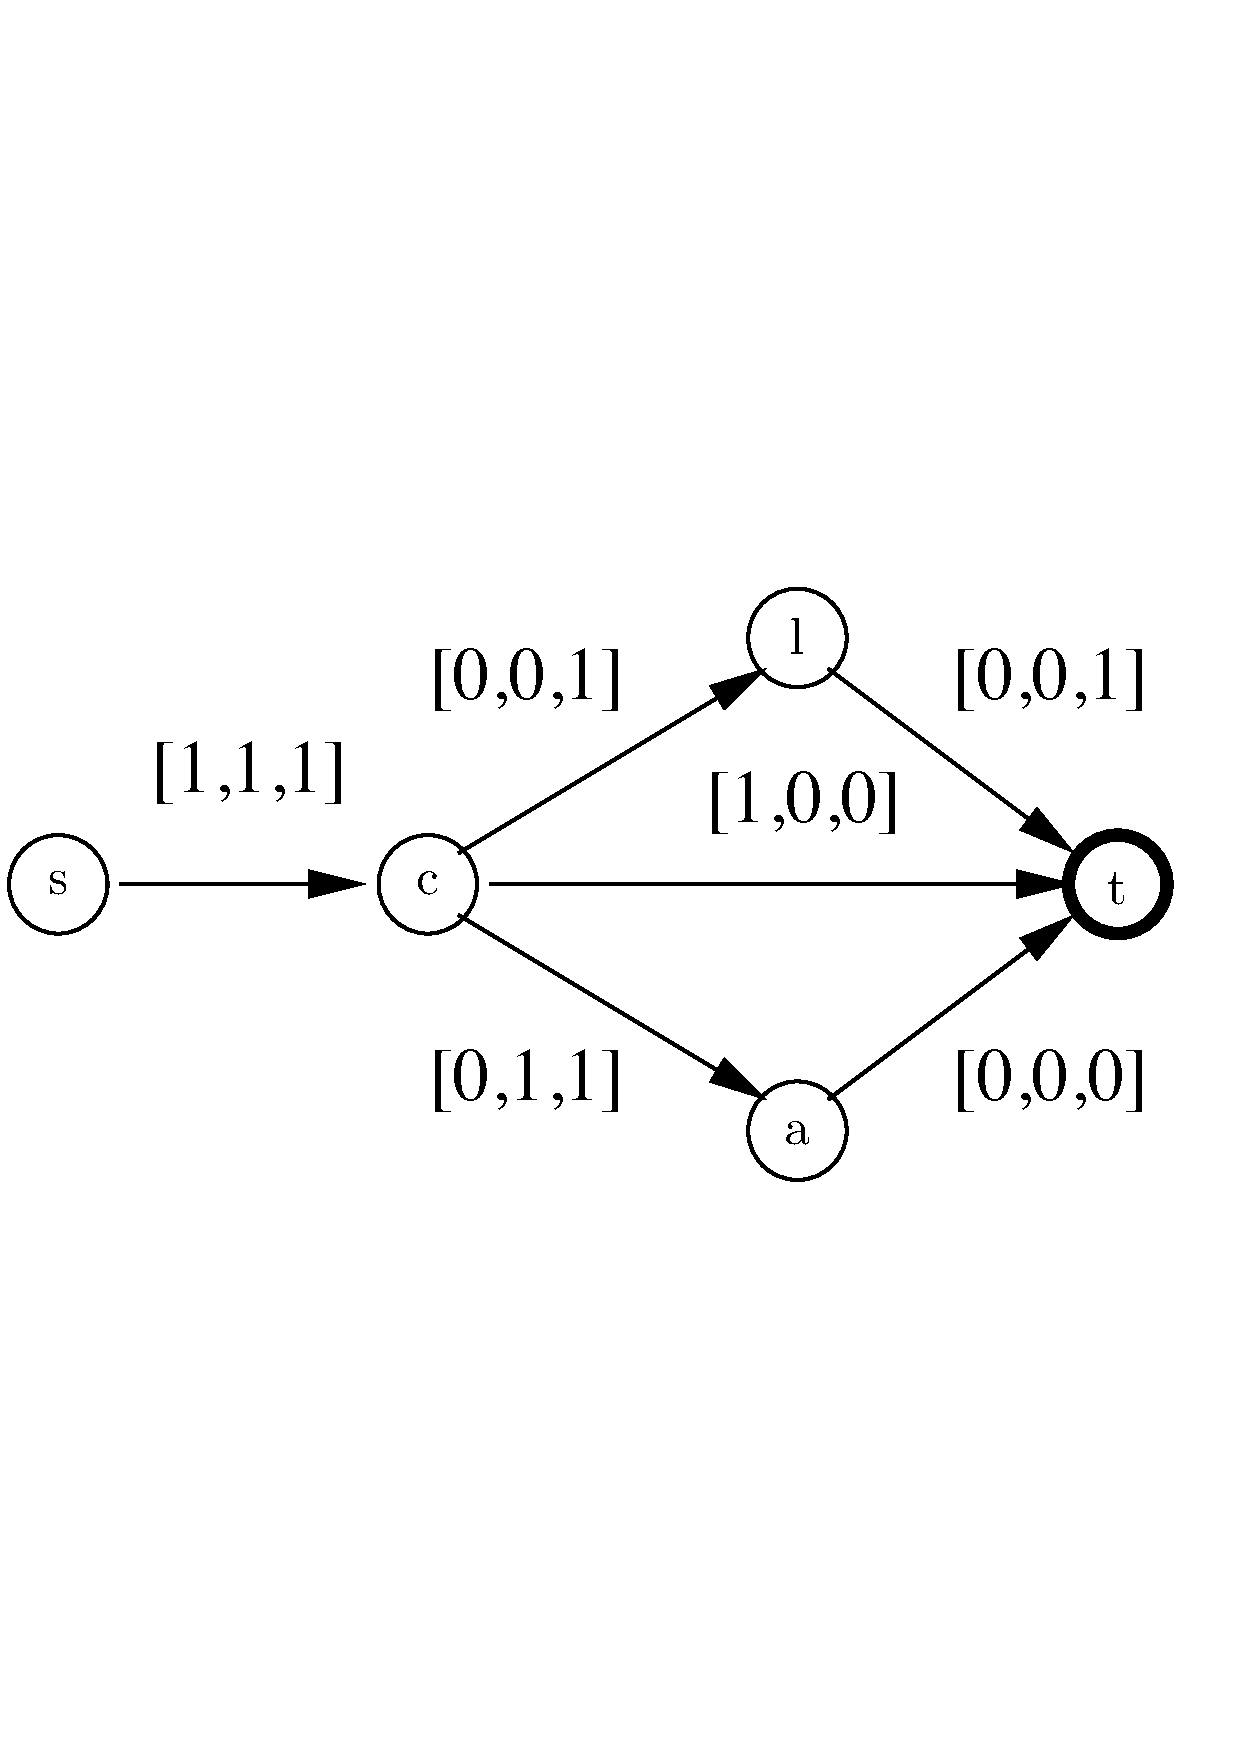
\includegraphics[width=0.3\textwidth]{figures/section3.pdf}
  \label{fig:sec3.1}
  \caption{Network graph}
\end{figure}

For the example on figure \ref{fig:sec3.1} assume $w=[1,2,0]$. There are three possible paths from $s$ to $t$.
\begin{itemize}
  \item The path $s\to c \to l \to t$ has a total cost of 3
  \item The path $s\to c \to t$ has a total cost of 4
  \item The path $s\to c \to a \to t$ has a total cost of 5
\end{itemize}

In the first attempt, a logical thing to do is to assume that $w$ is uniform. In other words $w = [q,q,q]$ with $q \in \mathbb{R}$. As a result, the agent will follow path $s\to c \to t$ because its predicted cost is the lowest. Then, it will receive $cost(s,c)=3$ and $cost(c,t)=1$  \\

By using linear algebra, the algorithm knows that
\begin{align}
  [w_1,w_2,w_3]\cdot [1,1,1] &=  3 \nonumber\\
  w_1+w_2+w_3 &=  3 \label{eqn:sec3.1}\\
  \nonumber\\
  [w_1,w_2,w_3] \cdot [1,0,0] &= 1 \nonumber\\
  \Rightarrow w_1 &=  1 \label{eqn:sec3.2}
\end{align}

After getting this information, the algorithm needs to decide the next path it will follow. Additionally, the $cost(a,t)$ must be equal to $0$ because $v_{at} = [0,0,0]$ and the algorithm can deduce $cost(c,a)$.
\begin{eqnarray*}
  cost(c,a) &=&  w \cdot [0,1,1] \\
  &=&  w \cdot ([1,1,1] - [1,0,0]) \\
  &=&  w \cdot [1,1,1] - w \cdot [1,0,0] \\
  &=&  w \cdot [1,1,1] - w \cdot [1,0,0] \\
  &=&  cost(s,c) - cost(a,t) \\
  &=&  3 - 1 \\
  &=&  2
\end{eqnarray*}
Therefore, it knows that the total cost of path $s \to c \to a \to t$ is $5$ which is not the minimum path.
Given that $v_{cl}$ is linearly independent of $v_{sc},v_{ct}$ it's impossible for the algorithm to know $cost(c,l)$ with the current information. Hence, it knows it doesn't know the total cost of $s \to c \to l \to t$. \\

In order to gather unknown information, in the next attempt the agent traverses path $s \to c \to l \to t$. After this, it will receive $cost(c,l) = 0$.
\begin{eqnarray}
  [w_1,w_2,w_3] \cdot [0,0,1] &=& 0 \nonumber\\
  w_3 &=& 0 \label{eqn:sec3.3}
\end{eqnarray}

By using equations (\ref{eqn:sec3.1}), (\ref{eqn:sec3.2}), (\ref{eqn:sec3.3}) the algorithm calculates $w=[1,2,0]$.
Now it is certain that the path with minimum total cost is $s \to c \to l \to t$. \\

In every attempt, this algorithm will either take the optimal path or take a path that contains a cost vector which is linearly independent to all the cost vectors previously explored. In the general case, with cost vectors of dimension $d$, the algorithm only needs to traverse $d$ edges with linearly independent cost vectors. Consequently, the number of $\bot$s is upper bounded by $d$.
